\documentclass[pdf]{beamer}
\mode<all>{\usetheme{Warsaw} \useoutertheme{default}}
\mode<handout>{\usecolortheme{seagull}}
%\usenavigationsymbolstemplate{}
\newtheorem{defn}[theorem]{Definition}

\title{Introduction to Commutative Algebra}
\subtitle{and affine algebraic varieties}
\author{Amal M}
\date{\today}

\begin{document}

%\AtBeginSection[]{
%\begin{frame}{Table of Contents}
%	\tableofcontents[currentsection]
%\end{frame}
%}

\begin{frame}
    \thispagestyle{empty}
    \titlepage
\end{frame}
\addtocounter{framenumber}{-1}

%\begin{frame}{Table of Contents}
%    \tableofcontents
%\end{frame}

%%%%%%%%%%%%%%%%%%%%%%%%%%%%%%%%%%%%%%%%%%%%%%%%%%

\section{Introduction}
\subsection{2 min}


\begin{frame}
    \frametitle{Introduction}
    The Plan
    \begin{itemize}
        \item Study undergraduate algebraic geometry 
        \item Read and do the exercies from Atiyah-Macdonald, Introduction to Commutative Algebra
        \item Read first chapter of Hartshorne's Algebraic Geometry
    \end{itemize}
\end{frame}


\section{Algebraic Varieties}
\subsection{3 min}

\begin{frame}
    \frametitle{Curves}
    $y^2 = x^3 - 3x + 5$ a polynomial in $\mathbb{R}[x,y]$. The set of zeros of this polynomial looks like this
    \begin{center}
        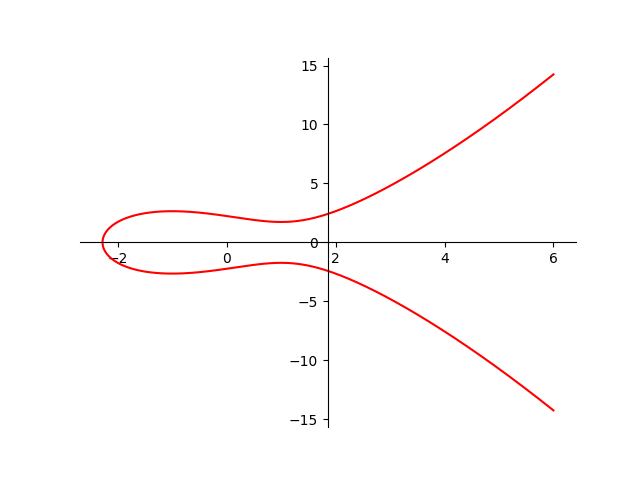
\includegraphics[height=2in]{ell_curv1.png}
    \end{center}
\end{frame}

\begin{frame}
    \frametitle{Polynomial Ring}
    Given a algebraicaly closed field $k$ we can form the polynomial ring in $n$ indeterminants
    $$k[x_1, \cdots, x_n]$$
    Every polynomial $p(x_1, \cdots, x_n) \in k[x_1, \cdots, x_n]$ can be thought of as a mapping from $k^n \rightarrow k$.
    We call $k^n$ the \textit{affine $n$-space} and denote it by $\mathbb{A}^n_k$.
\end{frame}

\begin{frame}
    \frametitle{Affine Algebraic Varieties}
    $S$ is a set of polynomial in $k[x_1, \cdots, x_n]$. $V(S)$ is points in $\mathbb{A}^n_k$ at which every polynomial in $S$ \textit{vanishes}. $V(S)$ is called the \textit{affine algebraic variety}.
\end{frame}    

\section{Nullstellensatz}
\subsection{5 min}

\begin{frame}
    \frametitle{The Coordinate Ring}
    Given a variety $V$ in $\mathbb{A}^n_k$ the \textit{ideal of a variety} is the ideal $I(V)$ which consists of all polynomials in $k[x_1, \cdots, x_n]$ that vanish on $V$. The Coordinate ring of a variety is the ring
    $$P(X) = k[x_1, \cdots, x_n]/I(X)$$
\end{frame}

\begin{frame}
    \frametitle{Hilbert's Nullstellensatz}
    \center Nullstellensatz means the theorem of zeros.
    \begin{center}
    \begin{tabular}{c | c}
        \large{\textbf{Algebra}} & \large{\textbf{Geometry}} \\
        $k[x_1, \cdots, x_n]$ & $\mathbb{A}^n_k \cong k^n$ \\
        $I(V)$ & $V(I)$ \\
        $(x - a_1, \cdots, x - a_n)$ & the point $(a_1, \cdots, a_n)$
    \end{tabular}
\end{center}
\end{frame}

\begin{frame}
    \frametitle{Algebraic - Geometry}
    There is a connection between geometric objects such as curves and the algebraical objects like a ring. 
\end{frame}

\begin{frame}
    \frametitle{Regular mappings}

    Given $f_1, \cdots, f_m \in k[x_1, \cdots, x_n]$ we have a polynomial mapping by $\phi(x) = (f_1(x) + \cdots + f_m(x))$ that takes $k^n \rightarrow k^m$.  

    \textit{Regular mappings} are maps between two varieties $X \subset k^n$ and $Y \subset k^m$ given by the restriction $\phi|_{X}: X \rightarrow Y$. 

\end{frame}

\section{Commutative Algebra}
\subsection{2 min}

\begin{frame}
    \frametitle{What sort of Commutative Algebra do we use?}
    What sort of commutative algebra machinery do we use?
    \begin{enumerate}
        \item Modules
        \item Tensor products
        \item Exact sequnces
        \item Direct Limits
    \end{enumerate}
\end{frame}

\section{Zariski Topology}
\subsection{3 min}

\begin{frame}
    \frametitle{Topology}
    Given an algebraic variety we can have a topology on it. One such topology is the Zariski Topology. 
    \begin{itemize}
        \item $X = \text{Spec}(A)$ is the prime spectrum of the ring $A$
        \item $V(E)$ are the closed sets on $X$
        \item $V(E)$ satisfies the three axioms for a topological space 
    \end{itemize}
\end{frame}

\begin{frame}
    \frametitle{Constructible Topology}
    We can have another topology called the Constructible Topology on $X = \text{Spec}(A)$.
    \begin{itemize}
        \item For each $f: A \rightarrow B$ we have $f^*: \text{Spec}(B) \rightarrow \text{Spec}(A)$
        \item The subset $f^*(\text{Spec}(B))$ of $\text{Spec}(A)$ is closed.
    \end{itemize}
\end{frame}

\begin{frame}
    When is the Zariski Topology and the Constructible Topology the same?
\end{frame}

\section{Presheaf and Sheaf}
\subsection{4 min}

\begin{frame}
    \frametitle{Presheaf and Sheaf}

    \begin{defn}
    Given an open set $U$ on a topological space $X$, the \textit{presheaf of rings}, $F$ on $X$ is defined as the following data
\begin{enumerate}
    \item To each open set $U$, a ring $F(U)$ is associated. The elements $f \in F(U)$ are called the \text{sections} of $F$ over $U$. The ring $F(X)$ is called a ring of \textit{global section}.  
    \item Let $U$ and $V$ be two open subsets of $X$ such that $V \subseteq U$. The ring homomorphim $\text{res}_{V,U}: F(U) \rightarrow F(V)$ associated with this mapping is called the \textit{restriction homomorphim}. If $f \in F(U)$ is a section, then $\text{res}_{V,U}(f)$ is called the restriction of $f$ and is denoted by $f|_{V}$.
    \end{enumerate}
    \end{defn}
\end{frame}

\begin{frame}
    \begin{defn}
Additionally, the restriction homomorphim must sastisfy the following conditions
\begin{enumerate}
    \item For each open set $U$ of $X$, the restriction homomorphim $\text{res}_{U,U}: F(U) \rightarrow F(U)$ is the identity homomorphim.
    \item If we have $W \subseteq V \subseteq U$ for three open sets, then $\text{res}_{W,V} \circ \text{res}_{V,U} = \text{res}_{W,U}$. That is we have the commutative diagram

\end{enumerate}
\end{defn}

\end{frame}

\begin{frame}
\begin{defn}
    Let  $U_i$ be a collection of open sets which cover the open set $U$. A presheaf $F$ is called a sheaf if given a collection of sections $f_i \in F(U_i)$ which satisfy  
    $$f_i |_{U_i \cap U_j} = f_j |_{U_i \cap U_j}, \forall i,j$$
   there exists a unique $f \in F(U)$ such that $f|_{U_i} = f_i$.
\end{defn}
 \end{frame}

 \section{Applications}
 \subsection{1 min}

 \begin{frame}
     \frametitle{How this any useful?}
     \begin{itemize}
         \item Algebraic geometry is used in Arithmetic geometry as there is a deep connection between algebraic geometry and number theoy
         \item Algebraic geometry is used in String Theory, eg, to study the properties of "curled up dimensions of spacetime"
         \item A recent brance of mathematical biology called Phylogenetic algebraic geometry
     \end{itemize}
\end{frame}

\section{Conclusion}

\begin{frame}
    \frametitle{Acknowledgement}
    Hwey Lewis
    Borat
\end{frame}
     
\end{document}
